\documentclass[a4paper,12pt]{article}
\usepackage{xcolor}
\usepackage{amsmath,amsfonts,amssymb}
\usepackage{geometry}
\usepackage{fancyhdr}
\usepackage{graphicx}
\usepackage{titlesec}
\usepackage{tikz}
\usepackage{booktabs}
\usepackage{array}
\usetikzlibrary{shadows}
\usepackage{tcolorbox}
\usepackage{float}
\usepackage{lipsum}
\usepackage{mdframed}
\usepackage{pagecolor}
\usepackage{mathpazo}   % Palatino font (serif)
\usepackage{microtype}  % Better typography
\usepackage{subfigure}
% \hypersetup{
%   colorlinks=true,
%   linkcolor=blue,
%   urlcolor=blue,
%   citecolor=blue
% }

% Page background color
\pagecolor{gray!10!white}

% Geometry settings
\geometry{margin=0.5in}
\pagestyle{fancy}
\fancyhf{}

% Fancy header and footer
\fancyhead[C]{\textbf{\color{blue!80}CS754 Assignment-5}}
% \fancyhead[R]{\color{blue!80}Saksham Rathi}
\fancyfoot[C]{\thepage}

% Custom Section Color and Format with Sans-serif font
\titleformat{\section}
{\sffamily\color{purple!90!black}\normalfont\Large\bfseries}
{\thesection}{1em}{}

% Custom subsection format
\titleformat{\subsection}
{\sffamily\color{cyan!80!black}\normalfont\large\bfseries}
{\thesubsection}{1em}{}

% Stylish Title with TikZ (Enhanced with gradient)
\newcommand{\cooltitle}[1]{%
  \begin{tikzpicture}
    \node[fill=blue!20,rounded corners=10pt,inner sep=12pt, drop shadow, top color=blue!50, bottom color=blue!30] (box)
    {\Huge \bfseries \color{black} #1};
  \end{tikzpicture}
}
\usepackage{float} % Add this package

\newenvironment{solution}[2][]{%
    \begin{mdframed}[linecolor=blue!70!black, linewidth=2pt, roundcorner=10pt, backgroundcolor=yellow!10!white, skipabove=12pt, skipbelow=12pt]%
        \textbf{\large #2}
        \par\noindent\rule{\textwidth}{0.4pt}
}{
    \end{mdframed}
}

% Document title
\title{\cooltitle{CS754 Assignment-5}}
\author{{\bf Saksham Rathi, Ekansh Ravi Shankar, Kshitij Vaidya}}
\date{}

\begin{document}
\maketitle
\textbf{Declaration:} The work submitted is our own, and
we have adhered to the principles of academic honesty while completing and submitting this work. We have not referred to any unauthorized sources, and we have not used generative AI tools for the work submitted here.

\section*{Question 1}

\begin{solution}{Solution}
  Here is the success probability image:
  \begin{figure}[H]
    \centering
    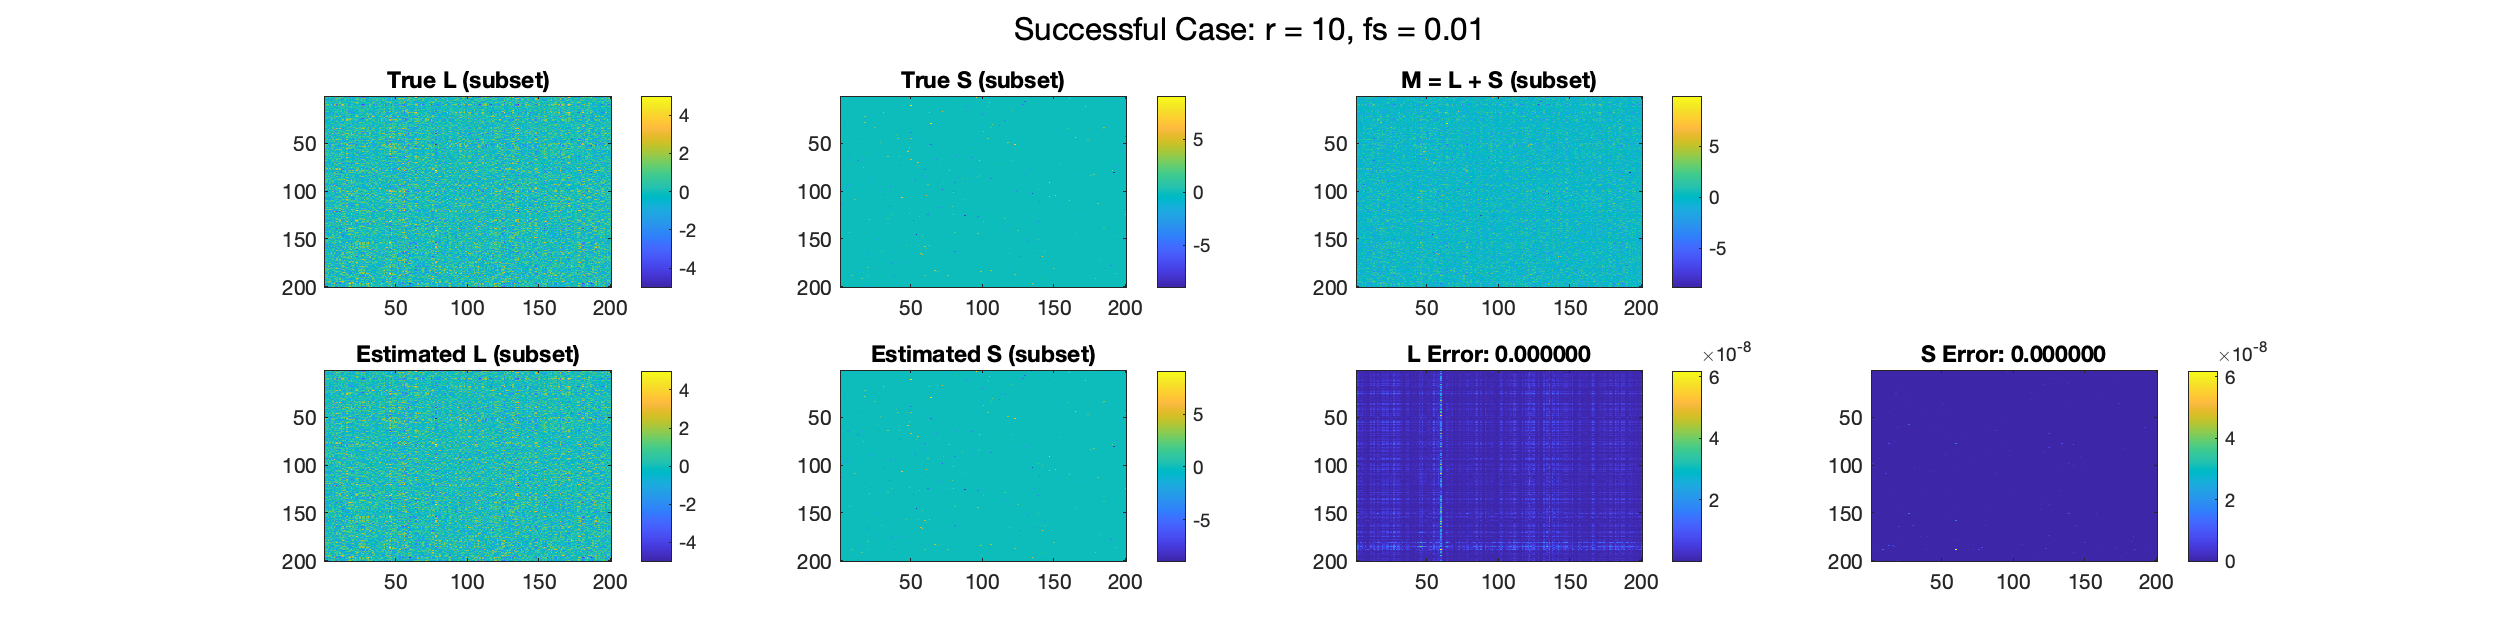
\includegraphics[width=\textwidth]{../code/success_probability_heatmap.png}
    \caption{Success Probability Heatmap}
  \end{figure}



  As we can see, mostly we are able to get a success of 1 for all 15 iterations, however for higher sparstiy fractions, or larger rank, we get lower success too. It also depends on the number of iterations for which we run our algorithm.

  \begin{figure}[H]
    \centering
    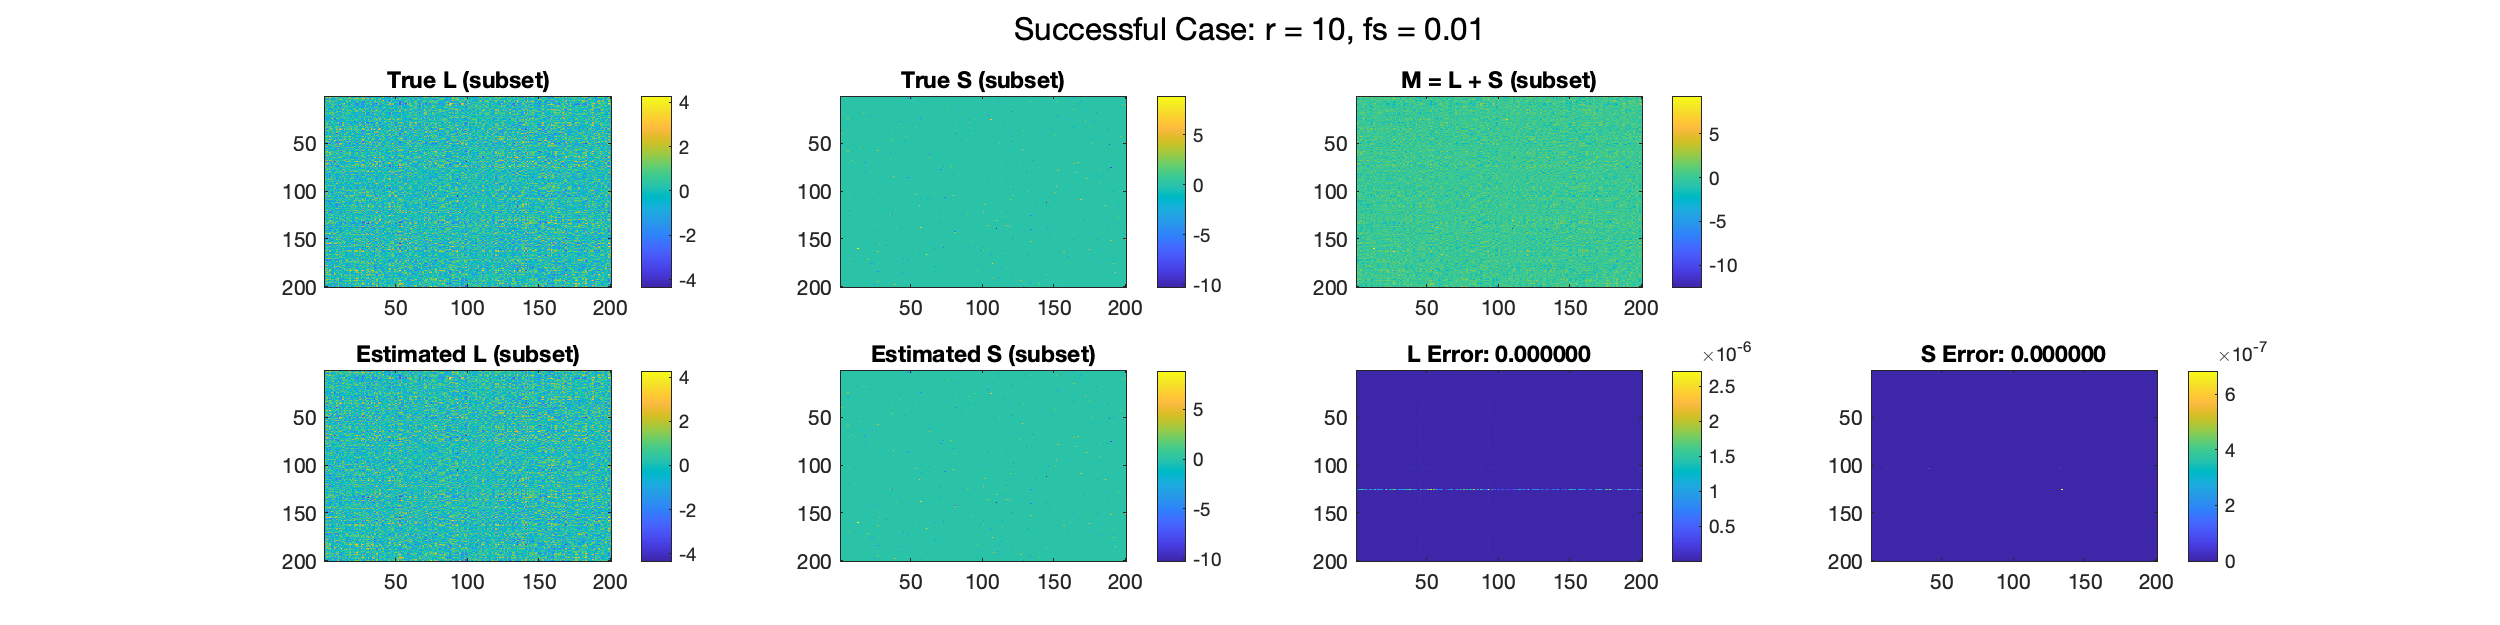
\includegraphics[width=\textwidth]{../code/successful_case_r10_fs0.01.png}
    \caption{Sucessful case}
  \end{figure}

  The above shows one of the successful cases.


  \begin{figure}[H]
    \centering
    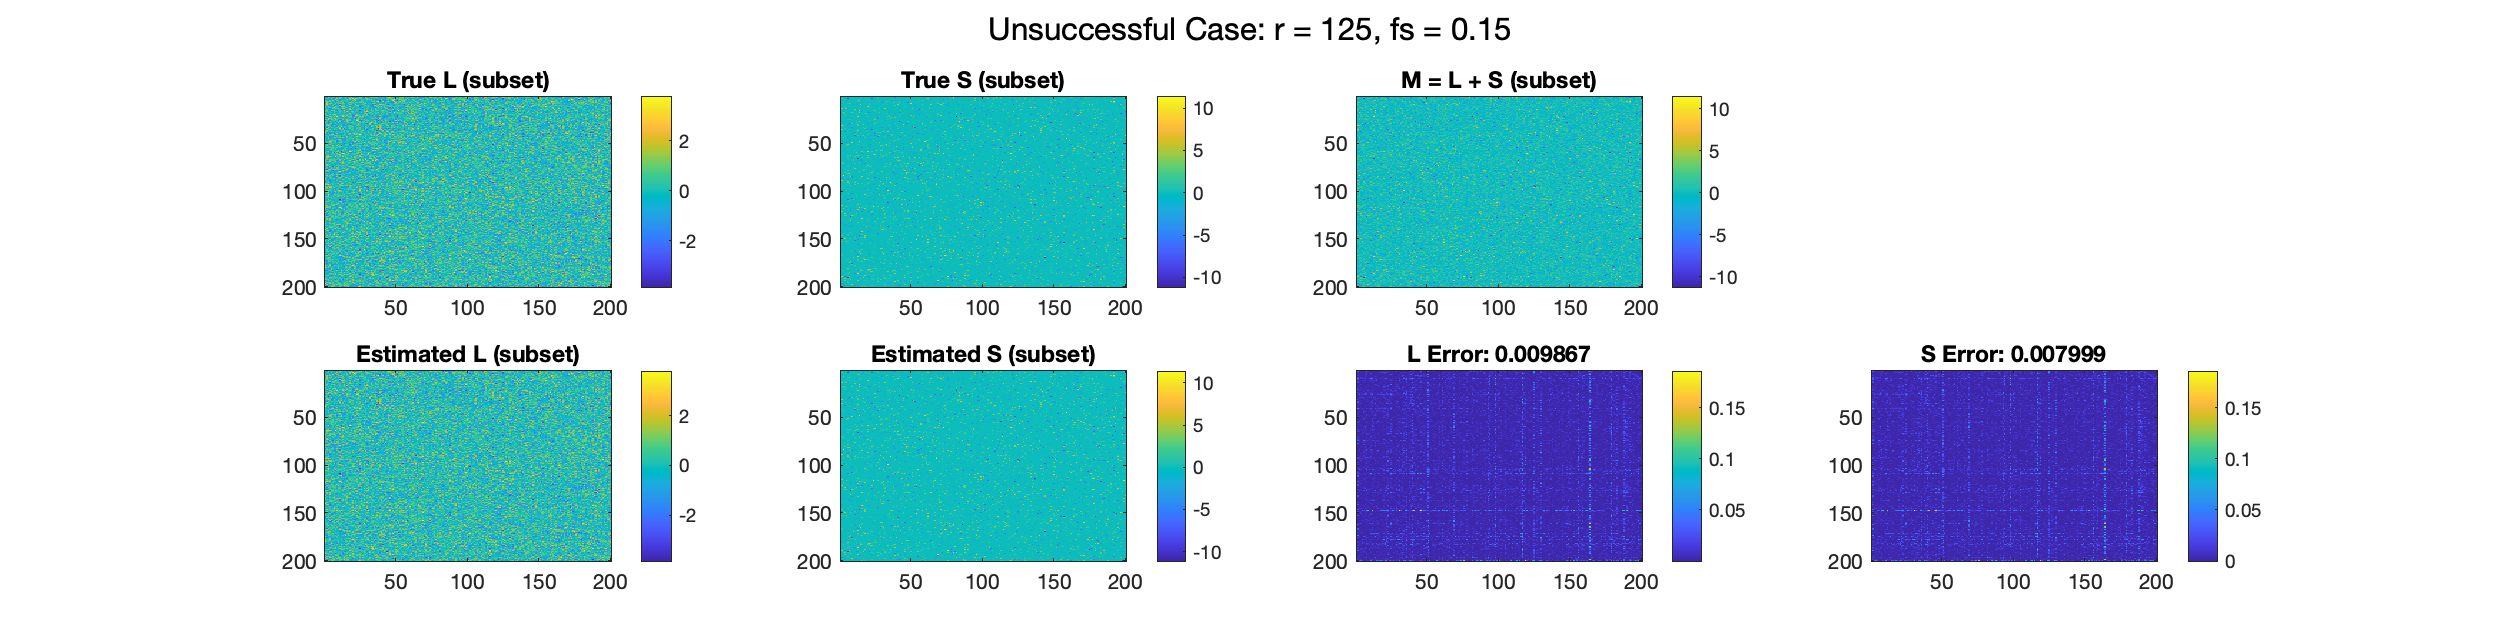
\includegraphics[width=\textwidth]{../code/unsuccessful_case_r125_fs0.15.png}
    \caption{Sucessful case}
  \end{figure}

  The above shows one of the unsuccessful cases.


  As we can see in the unsuccessful case, there is a lot of noise in L, and the error is larger enough.


\end{solution}




\end{document}
